\documentclass[a4paper]{article}

% Set margins
\usepackage[hmargin=2.5cm, vmargin=3cm]{geometry}

\frenchspacing

% Language packages
\usepackage[utf8]{inputenc}
\usepackage[T1]{fontenc}
\usepackage[magyar]{babel}

% AMS
\usepackage{amssymb,amsmath}

% Graphic packages
\usepackage{graphicx}

% Colors
\usepackage{color}
\usepackage[usenames,dvipsnames]{xcolor}

% Listings
\usepackage{listings}

% Question
\newenvironment{question}[1]
{\noindent\textcolor{OliveGreen}{$\circ$ \textit{#1}}

\smallskip

\color{Gray}

}{\bigskip}

% Task
\newenvironment{task}[1]
{\noindent\textcolor{RoyalBlue}{$\circ$ \textit{#1}}

\smallskip

\color{Gray}

}{\bigskip}

% Notification
\newenvironment{notification}[1]
{\noindent\textcolor{Peach}{$\circ$ \textit{#1}}

\smallskip

\color{Gray}

}{\bigskip}

% Problem
\newenvironment{problem}[1]
{\noindent\textcolor{OrangeRed}{$\circ$ \textit{#1}}

\smallskip

\color{Gray}

}{\bigskip}

% Solution
\newenvironment{solution}
{\color{RoyalBlue}}{\bigskip}

% Comment
\newenvironment{comment}
{\color{Green}}{\bigskip}

\lstset{% setup listings
        framexleftmargin=16pt,
        framextopmargin=6pt,
        framexbottommargin=6pt, 
        frame=single, rulecolor=\color{black}
}

%===============
\begin{document}
%===============

\definecolor{codebg}{rgb}{0.99,0.99,0.99}
\lstset{backgroundcolor=\color{codebg}}

\begin{center}
    \Huge \textbf{Programtervezési ismeretek}
    
	\bigskip
	
	\Large gyakorlat
\end{center}

\bigskip

%=====================
\section*{1. Halmazok, számrendszerek}
%---------------------

\begin{enumerate}

\item

Tekintsük az $A = \{p, q, r\}$ és $B = \{5, 8\}$ halmazokat!
\begin{itemize}
	\item Írjuk fel az $A \times A, A \times B, B \times A, B \times B$ Déscartes szorzatokat!
	\item Írjuk fel a $2^A$, $2^B$ halmazokat!
	\item A halmazok kiszámítása előtt határozzuk meg azok elemszámát!
\end{itemize}

\begin{comment}
A Déscartes szorzat nem kommutatív, asszociatív.

A párok tagjai nem cserélhetők fel, viszont a párok a halmazon belül igen.

A $2^A$ helyett szokták még a $\mathcal{P}(A)$ jelölést használni (mint \textit{power}).
\end{comment}

\item

Számítsuk ki az $52 \cdot 149$ szorzatot orosz-paraszt módszerrel!
\begin{itemize}
	\item Ellenőrízzük kézzel kiszámítva a szorzatot!
	\item Számítsuk ki $149 \cdot 52$ formában is!
\end{itemize}

\begin{solution}
\begin{tabular}{|c|c|c|c|}
szorzandó & szorzó & szorzó páratlan? & szorzat \\
\hline
52 & 149 & igen & 0 + 52 \\
104 & 74 & nem & 52 \\
208 & 37 & igen & 52 + 208 = 260 \\
416 & 18 & nem & 260 \\
832 & 9 & igen & 260 +832 = 1092 \\
3328 & 2 & nem & 1092 \\
6656 & 1 & igen & 1092 + 6656 = \textbf{7748} \\
\hline
& 0 & & \\
\end{tabular}
\end{solution}

\begin{comment}
Megvitatni, hogy ez a módszer egyszerűbb, vagy bonyolultabb-e, mint a hagyományos szorzási módszer. $\Rightarrow$ \textit{Gépeknek egyszerűbb}
\end{comment}

Számítsuk ki a $63 \cdot 154$ szorzatot! $\Rightarrow 9702$

\item

Számítsuk ki a következő kifejezések értékét!

\begin{comment}
$$
\lfloor x \rfloor = \max_{k \leq x} k, \quad x \in \mathbb{R}, k \in \mathbb{Z}
\hskip 3cm
\lceil x \rceil = \min_{k \geq x} k, \quad x \in \mathbb{R}, k \in \mathbb{Z}
$$

$$
\text{Round}(x) = \left\lfloor x + \dfrac{1}{2} \right\rfloor,
\quad x \in \mathbb{R}
\hskip 3cm
\{x\} = x - \lfloor x \rfloor, \quad x \in \mathbb{R}
$$

$$
a \text{ div } b = \left\lfloor \dfrac{a}{b} \right\rfloor
\hskip 2cm
a \text{ mod } b = \begin{cases}
a, & \text{ha } b = 0, \\
a - \left\lfloor \dfrac{a}{b} \right\rfloor \cdot b, & \text{ha } b \neq 0. \\
\end{cases}
\hskip 1cm
a \text{ mod } 1 = \{a\}
$$
\end{comment}

Mi a függvények értelmezési tartománya és értékkészlete?

\begin{itemize}
	\item Egészrész függvény:
		$\lceil 8.1 \rceil$,
		$\lfloor 0.2 \rfloor$,
		$\left\lfloor \dfrac{52}{7} \right\rfloor$,
		$\lfloor -6.5 \rfloor$,
		$\lceil -7.51 \rceil$
	\item Kerekítő függvény:
		$\text{Round}(8.1)$,
		$\text{Round}(0.2)$,
		$\text{Round}\left( \left\lfloor \dfrac{52}{7} \right\rfloor \right)$,
		$\text{Round}(-6.5)$,
		$\text{Round}(-7.51)$
	\item Törtrész függvény:
		$\{ 8.1 \}$,
		$\{ 0.2 \}$,
		$\left\{ \dfrac{52}{7} \right\}$,
		$\{ -6.5 \}$,
		$\{ -7.51 \}$
	\item Egész hányados képzése, div művelet:
		27 div 5, 12 div 0, 21 div -9, -11 div 3, -20 div -7
	\item Egész maradék képzése, mod művelet:
		27 mod 5, 12 mod 0, 21 mod -9, -11 mod 3, -20 mod -7
\end{itemize}

\begin{solution}
Elegendő visszahelyettesíteni a definíciókba.
\end{solution}

Megnézni az előjeles és előjel nélküli változatok eredményeit, például $31 \div 7$ és $31 \mod 7$ esetén!

\item

Egész szám adatstruktúra

$$
c_n, c_{n-1}, \ldots, c_1, c_0 \quad 0 \leq c_k < b, b \geq 2
$$

$$
x = c_n \cdot b^n + c_{n-1} \cdot b^{n-1} + \cdots + c_1 \cdot b^1 + c_0 \cdot b^0 = \sum_{i=1}^n c_n \cdot b^n
$$

\begin{itemize}
	\item Milyen értéket jelölnek a következő számalakok?
$$
7352_{10}, 10111010_{2}, 25136_{7}, 8FB2_{16}, 121020_{3}, 444_{5}, 5566_{8}
$$
\begin{solution}
Felírni az $A-F$ hexadecimális számjegyek megfelelőit!
\end{solution}
	\item Írjuk fel a 2016-ot 2, 3, 7, 8, 10, 11, 16-os számrendszerben!
	
\begin{solution}
Megmutatni a 2, 4, 8 és 16 számrendszerek közötti könnyebb átjárhatóságot!
\end{solution}

	\item Ellenőrízzük helyiértékesen és Horner sémával!
\end{itemize}

\item

Adjuk össze a következő értékeket a megfelelő számrendszerekben!

\begin{align*}
&1011101_{2} + 11001_{2} \\
&2133_{4} + 321_{4} \\
&43705_{8} + 1162_{8} \\
&30112_{5} + 4040_{5} \\
\end{align*}

\item

Mennyi számjegyből fog állni a 62982 szám 2, 3, 6, 10, 15, 16-os számrendszerben?

$$
n + 1 = \left\lfloor \log_b x \right\rfloor + 1
$$

\begin{comment}
Hangsúlyozni, hogy a számjegyek száma az $n + 1$.

Kitérni arra, hogy hogyan lehet tetszőleges természetes szám alapú logaritmust számolni.

* Megmutatni, hogy az orosz-paraszt módszer táblázatában a sorok számát ezzel lehet számolni, mivel a harmadik oszlop a kettes számrendszerbeli alakot adja, csak más reprezentációval.
\end{comment}

\end{enumerate}

%=====================
\section*{2. Számábrázolás, negatív és lebegőpontos számok}
%---------------------

Feladatok az előző témakörhöz
\begin{itemize}
\item $A = \{2, 3, 4\}, B = \{p, q\}, |A^7 \times B^8| = ?$
\item Az alsó- és felsőegészrész függvény ábrázolása.
\item A törtrész függvény ábrázolása.
\item Megvizsgálni, hogy teljesül-e a következő:
$$
\text{Round}(x) =
\left\lfloor x + \dfrac{1}{2} \right\rfloor =
\left\lceil x - \dfrac{1}{2} \right\rceil
$$
\end{itemize}

\begin{enumerate}

\item

Egészek ábrázolása

Számábrázolási tartományok

\begin{solution}
\begin{tabular}{|c|c|c|}
byte-ok száma & előjel nélküli & előjeles \\
\hline
1 & $[0, 255]$ & $[-128, 127]$ \\
2 & $[0, 65535]$ & $[-32768, 32767]$ \\
3 & $[0, 2^{24} - 1]$ & $[-2^{23}, 2^{23} - 1]$ \\
4 & $[0, 2^{32} - 1]$ & $[-2^{31}, 2^{31} - 1]$ \\
\hline
$k$ bit esetén & $[0, 2^k - 1]$ & $[-2^{k-1}, 2^{k-1}-1]$ \\
\end{tabular}
\end{solution}

\begin{comment}
A 16777215 az a kijelzőknél emlegetett 17 millió színt jelöli.

A $2^{32}$ a harminckét bites címzés miatt lehet ismerős.
\end{comment}

\item

Negatív egészek ábrázolása, kettes komplemens

\begin{solution}
Bemutatni az algoritmust az $1011100_2$ értéken. 

\textit{(Ezen azért jó, mert kicsi a számérték, vannak a végén nullák, és nem tölt ki egy byte-ot.)}

Megmutatni, hogy az összeg valóban 0-át ad (egy átviteli bittel a legnagyobb helyiérték után).
\end{solution}

Mennyi byte szükséges a -281, -512, -14890 számok ábrázolásához?

\item

Törtek átírása
\begin{itemize}
	\item Írjuk át a $0.110101_2$, $0.1201_3$ és $0.AB1E_{16}$ értékeket tizes számrendszerbe!
	\item Írjuk át a 0.1, 0.15 és 0.625 értékeket kettes és tizenhatos számrendszerbe!
\end{itemize}

\begin{solution}
Megmutatni a helyiértékes és a Horner-sémás átírást is!
\end{solution}

\item

Váltsuk át a 14889 és -2488 számokat kettes számrendszerbe!
\begin{itemize}
	\item Mennyi bitből fog állni?
	\item Adjuk össze őket kettes számrendszerben!
	\item Az összeget számoljuk vissza 10-es számrendszerbe, és ellenőrízzük!
\end{itemize}

\item

Írjuk fel kettes számrendszerbe a következő értékeket!
$$
0.42578125_{10}, \quad
0.70312_{10}, \quad
0.74_{10}, \quad
0.14062_{10}, \quad
0.15_{10}, \quad
0.ABCD_{16}
$$
Ellenőrízzük helyiértékesen és Horner sémával is!

\item

Lebegőpontos számok ábrázolása!

Ábrázoljuk egyszeres lebegőpontos számábrázolással a következő értékeket!
$$
149.765625, \quad
-0.7, \quad
7513.625, \quad
0.41, \quad
9.7
$$

\item

Számítsuk ki, hogy milyen értékeket ábrázolnak a következő byte-ok egyszeres lebegőpontos ábrázolást feltételezve!
$$
8AC20000, \quad FE90C000, \quad 14011000, \quad C5D20000, \quad 7D3C8000
$$

\item

Ha egy szám 61 jegyű kettes számrendszerben, akkor hány jegyű lesz 16 és 10-es számrendszerben?

\medskip

Ha egy szám 9 jegyű 16-os számrendszerben, akkor hágy jegyű lesz 10-esben és kettesben?

\item

Mennyi byte-on lehet ábrázolni a Neptun kódokat?

\medskip

Mi lenne, ha nem lennének benne számjegyek?

\item

Egyszeres pontosságú lebegőpontos számábrázolás

-51000.3046875, 0.9, 3.6, 4.78125, 3.141592
85EA0000, ABCD0000, FCA20000, 90909090

\item

Adjuk meg a végtelen értékeket egyszeres pontossággal!

\medskip

Milyen érték a 7F801000?

\item

Egyszeres pontossággal milyen értékeket ábrázolnak a következő byte-ok?
$$
66 1B 0C 42, \quad
66 1B 0A 1F
$$

\item

Töltsük ki az alábbi táblázatot!

\begin{tabular}{|l|c|c|c|}
duplaszó hexában & \texttt{FA00AB87} & \texttt{10203040} & \texttt{DEADBEEF} \\
\hline
előjel nélküli & & & \\
előjeles & & & \\
egyszeres lebegőpontos & & & \\
\hline
\end{tabular}

\end{enumerate}


%=====================
\section*{3. Logikai értékek és műveletek}
%---------------------

Feladatok az előző témakörhöz

\begin{itemize}
\item Ábrázoljuk a $-75.1796875$ értéket egyszeres lebegőpontos számábrázolással!

\begin{solution}
Hexadecimálisan a \texttt{C2965C00} byte-okon ábrázolható.
\end{solution}

\item Milyen számértéket ábrázolnak a \texttt{BB6D7000} byte-ok egyszer lebegőpontos ábrázolást feltételezve?

\begin{solution}
A $-0.0036230087$ értéket ábrázolja. (A kitevő $-9$, az eredmény $\dfrac{\text{ED7}_{16}}{2^{20}}$ formában számolható.)
\end{solution}

\item Írjuk fel egyszeres lebegőpontos számábrázolással a 0-át és a végtelent, illetve adjunk példát \textit{denormalizált} és \textit{nem szám}ra.

\begin{solution}
\begin{tabular}{ll}
+0 & \texttt{00 00 00 00} \\
-0 & \texttt{80 00 00 00} \\
+Inf & \texttt{7F 80 00 00} \\
-Inf & \texttt{FF 80 00 00} \\
Den & \texttt{00 01 00 00} \\
NaN & \texttt{7F 80 10 00} \\
\end{tabular}
\end{solution}

\begin{comment}
0 $\rightarrow$ denormalizált, ha nem nulla a szignifikáns.

$\infty \rightarrow$ NaN, ha nem nulla a szignifikáns.
\end{comment}

\end{itemize}

\begin{enumerate}

\item

Logikai műveletek

\begin{itemize}
	\item Milyen logikai műveleteket ismerünk?
	\item Melyek unárisak és melyek binárisak ezek közül?
	\item Mennyi lehetséges unáris és bináris művelet van?
	\item Írjuk fel a logikai műveletek művelettábláit!
	
	(Az $\wedge, \vee, \oplus, \leftrightarrow, \rightarrow, \downarrow, |$ műveleteket külön megnézni!)
\end{itemize}

\begin{solution}
A művelettáblákba itt még elég, ha \textit{i} és \textit{h} betűk kerülnek.
\end{solution}

\item

Írjuk fel a 3 bemenetes többségi szavazás diszjunktív normál formáját, és rajzoljuk fel a kapuáramkört!

\begin{solution}
Jelölje $a$, $b$ és $c$ az egyes szavazatokat. Ekkor a szavazógép igazságtáblája a következőképpen néz ki.

\begin{center}
\begin{tabular}{|ccc|c|}
$a$ & $b$ & $c$ & $f(a, b, c)$ \\
\hline
0 & 0 & 0 & 0 \\
0 & 0 & 1 & 0 \\
0 & 1 & 0 & 0 \\
0 & 1 & 1 & 1 \\
1 & 0 & 0 & 0 \\
1 & 0 & 1 & 1 \\
1 & 1 & 0 & 1 \\
1 & 1 & 1 & 1 \\
\hline
\end{tabular}
\end{center}

A diszjunktív normálforma felírásához tekintsük azokat a sorokat, amelyekben $f(a, b, c) = 1$. (Ezek a 4., 6., 7. és 8. sorok.) Írjuk fel elemi konjunkciókat a változókból úgy, hogy ahol a változó értéke $0$ az adott sorban, ott a változó negáltját szerepeltessük. Az elemi konjunkciók a következők lesznek.
$$
\overline{a} \wedge b \wedge c, \quad
a \wedge \overline{b} \wedge c, \quad
a \wedge b \wedge \overline{c}, \quad
a \wedge b \wedge c
$$
A normál diszjunktív normálformát ezeknek az elemi konjunkcióknak a diszjunkciójából kapjuk.
$$
f(a, b, c) =
(\overline{a} \wedge b \wedge c) \vee
(a \wedge \overline{b} \wedge c) \vee
(a \wedge b \wedge \overline{c}) \vee
(a \wedge b \wedge c)
$$

\end{solution}

\item

Fejezzük ki az antivalencia, implikáció és az ekvivalencia műveleteket az $\wedge$, $\vee$ és negáció műveletekkel!

\begin{align*}
x \oplus y &\equiv (\overline{x} \wedge y) \vee (x \wedge \overline{y}) \\
x \rightarrow y &\equiv \overline{x} \vee y \\
x \leftrightarrow y &\equiv (x \wedge y) \vee (\overline{x} \wedge \overline{y})
\end{align*}

\begin{solution}
Érdemes inkább levezetni őket igazságtáblával!
\end{solution}

\item

Tervezzünk 5 bemenetes automatát, amely a maximumot adja vissza!

\begin{solution}
\begin{itemize}
\item Fel kell rajzolni az 5 bemenetes kapuáramkör be- és kimenetét.
\item Meg kell nézni, hogy 2 bemenet elején hogy nézne ki.
\item Kettessével össze kell vagyolni a bemeneteket.
\item Ki kell írni a kifejezést, és a kapuáramkörnek megfelelően be kell zárójelezni.
\item Meg lehet mutatni, hogy a minimum is hasonlóképpen alakulna.
\end{itemize}
\end{solution}

\item

Tervezzünk kapuáramkört az $\wedge$, $\vee$ és negáció műveletekkel az $u = f(x, y, z) = (x \oplus y) \rightarrow z$ logikai függvényhez és írjuk fel a diszjunktív normál formáját!

\begin{solution}

\begin{center}
\begin{tabular}{|ccc|c|c|}
$x$ & $y$ & $z$ & $x \oplus y $ & $(x \oplus y) \rightarrow z$ \\
\hline
0 & 0 & 0 & 0 & 1 \\
0 & 0 & 1 & 0 & 1 \\
0 & 1 & 0 & 1 & 0 \\
0 & 1 & 1 & 1 & 1 \\
1 & 0 & 0 & 0 & 1 \\
1 & 0 & 1 & 0 & 1 \\
1 & 1 & 0 & 1 & 0 \\
1 & 1 & 1 & 1 & 1 \\
\hline
\end{tabular}
\end{center}
A diszjunktív normálforma felírásához a 3. és 7. sort leszámítva minden sort figyelembe kell venni. A DNF a következő lesz.
$$
f(x, y, z) =
(\overline{x} \wedge \overline{y} \wedge \overline{z}) \vee
(\overline{x} \wedge \overline{y} \wedge z) \vee
(\overline{x} \wedge y \wedge z) \vee
(x \wedge \overline{y} \wedge \overline{z}) \vee
(x \wedge \overline{y} \wedge z) \vee
(x \wedge y \wedge z)
$$
\end{solution}

\end{enumerate}

%=====================
\section*{4. gyakorlat}
%---------------------

\begin{enumerate}

\item

Készítsünk egész összeadót félösszeadókból!

\begin{solution}
\begin{itemize}
\item Érdemes felírni a félösszeadó és a teljes összeadó igazságtábláját, és felrajzolni hozzá a kapuáramköröket!
\end{itemize}
\end{solution}

\item

Írjuk fel az $\wedge$, $\vee$, $\neg$, $\rightarrow$, $\oplus$, $\leftrightarrow$, $\downarrow$ műveleteket \textit{Scheffer vonás}sal, és rajzoljuk fel a kapuáramköröket \textit{NAND} kapukkal!

\begin{solution}
Az $\oplus$ ábráját egyben felrajzolni úgy, hogy utána az élekre lehessen írni, hogy mi az aktuális részeredmény, és így belátni, hogy valóban jó eredményt ad!
\end{solution}

\item

Lássuk be a következőket!

\begin{solution}
Felírni hozzá a műveletekre vonatkozó azonosságokat!

Megemlíteni, hogy igazszágtáblával is lehetne bizonyítani, viszont az több változó esetén már nem lenne praktikus.
\end{solution}

$x \wedge (y \oplus z) \equiv (x \wedge y) \oplus (x \wedge z)$

$(p \wedge q \wedge r) \rightarrow s \equiv p \rightarrow (q \rightarrow (r \rightarrow s))$

$(p \wedge (p \rightarrow q)) \rightarrow q \equiv 1$

$(a | b) \oplus (a \downarrow b) \equiv a \oplus b$

\item

Igazoljuk a következő egyenlőségeket!

$\overline{A \setminus B} \cap (\overline{A} \cup \overline{B}) = \overline{A}$

$A \cap (\overline{A \setminus B}) = A \cap B$

$\overline{(P \setminus Q) \bigtriangleup R} =
(\overline{R} \cup P) \cap (\overline{R} \cup \overline{Q}) \cap (\overline{P} \cup Q \cup R)$

$A \setminus (B \setminus (C \setminus D)) =
A \cap (\overline{B} \cup \overline{C} \cup D)$

\end{enumerate}

%=====================
\section*{5. gyakorlat}
%---------------------

\begin{enumerate}

\item

Tervezzünk 4 bemenetes paritás ellenörző automatát!

\item

Vizsgáljuk meg az alábbi azonosságokat!

$a \rightarrow ((b|a) \wedge \overline{b})
\equiv a$

$\overline{a \wedge \overline{b \wedge \overline{c \wedge d}}} \equiv ?$

$\overline{(x \oplus y) \rightarrow z} \equiv
(x \wedge \overline{y} \wedge \overline{z}) \vee
(\overline{x} \wedge y \wedge \overline{z})$

$(a|b) \downarrow (c|d) \equiv
(d|a) \downarrow (c|b)$

\item

Írjuk fel az $f(x_1, x_2, x_3) = (x_1 \oplus x_3) \wedge (x_2 \rightarrow x_1)$ DNF-jét! Rajzoljunk kapuáramkört!

...hasonlóképp a $g(x_1, x_2, x_3) = (x_2 \vee x_3) \leftrightarrow (x_1 \wedge x_2)$-vel.

\item

Mennyi olyan halmazpár van, amelyeknek a metszete $\{a, b, c\}$ uniója pedig $\{a, b, c, d, e, f\}$?

\item

Igazoljuk a következő egyenlőségeket!

$C \cap (A \bigtriangleup B) = A \cap \overline{B} \cap C$, ha $B$ és $C$ diszjunkt.

$(K \cap L) \setminus (K \setminus M) = K \cap L \cap M$

$(K \setminus L) \setminus M = (K \setminus M) \setminus (L \setminus M)$

$\overline{P \bigtriangleup Q} \setminus R = (\overline{P} \cup Q) \cap (P \cup \overline{Q}) \cap \overline{R}$

\item

Tekintsük az $A = (-5; 4]$ és a $B = [3; 9)$ intervallumokat. Határozzuk meg a következő kifejezések értékét:
$A \cup B, A \cap B, A \setminus B, B \setminus A, A \bigtriangleup B, A \times B, 2^A, 2^B$.

\item

Írjuk fel a $2^{2^{\{a, b\}} \setminus \{b\}}$ halmaz elemeit!

\medskip

Van-e jelentősége annak, hogy $\{b\}$ szerepel, nem pedig csak $b$?

\item

Ha $|H| = 60, A \subset H, B \subset H, |A| = 48, |B| = 32$ akkor mennyi lesz $|A \cup B|$ és $|A \cap B|$?

\end{enumerate}

%=====================
\section*{6. gyakorlat}
%---------------------

\begin{enumerate}

\item

Karakterkódolás

\begin{solution}
\begin{itemize}
\item Fix és változó hosszúságú kódolás előnyei, hátrányai.
\item UTF-8 kódolás, tárolási mód
\item Nem egyértelmű megadás (szabvány szerint tiltott)
\item Szövegek átalakítása számokká.
\end{itemize}
\end{solution}

\item

Alakítsuk át a következő unicode szimbólumokat UTF-32 és UTF-8 kódolásúra!

U+0048, \quad U+082C, \quad U+10EE65, \quad U+9AF1

\begin{solution}
Átírni bináris alakba. Megszámolni, hogy mennyi bit szükséges az ábrázoláshoz. Meghatározni az alapján a byte-ok számát. Felrajzolni a keretet formátumnak megfelelően. Kitölteni a bit-eket. Visszaírni hexadecimális alakba a byte-okat.
\end{solution}

\item

Adjuk meg az első és az utolsó érvényes unicode kódot a byte-ok számának megfelelően!

\begin{solution}
\begin{center}
\begin{tabular}{|c|c|l|l|}
byte-ok száma & felhasználható bitek száma & első kód & utolsó kód \\
\hline
1 & 7 & U+0000 & U+007F \\
\hline
2 & 11 & U+0080 & U+07FF \\
\hline
3 & 16 & U+0800 & U+FFFF \\
\hline
4 & 21 & U+10000 & U+1FFFF \\
\hline
5 & 26 & U+20000 & U+3FFFFFF \\
\hline
6 & 31 & U+4000000 & U+7FFFFFFF \\
\hline
\end{tabular}
\end{center}
\end{solution}

\item

Szövegláncok/sztringek

Hogyan tudunk sztringeket tárolni? \textit{(C, Pascal, előnyök, hátrányok)}

\begin{solution}
Felírni egymás mellé a két fajta konvenciót, és a következő szempontokat érdemes megtárgyalni:
\begin{itemize}
\item szövegek maximális hossza,
\item hossz meghatározása,
\item ábrázolható karakterek,
\item konkatenálás költsége,
\item hibatűrés (pl.: termináló 0 lemarad, vagy több van).
\end{itemize}

Szövegszerkesztő megvalósítása. $\rightarrow$ A karakter beszúrásánál vagy törlésénél az egész buffer átméretezése túl költséges lenne.
\end{solution}

Milyen attribútumai és műveletei vannak a sztringeknek?

\begin{solution}
Az attribútumos jelölésmódra külön kitérni!
\end{solution}

A konkatenáció művelete kommutatív, asszociatív-e?

\begin{solution}
Nem. Igen.
\end{solution}

\item

Adott egy tömb a memóriában, amelynek elemei 48 bájtosak. Az 50-edik elem a tömbelem 9. bájtjának 5. bitje hanyadik bitje lesz a tömbnek?
\begin{itemize}
	\item Vizsgáljuk külön a 0 és 1 kezdőindexek eseteit!
	\item Hogyan tudnánk felírni általánosan, ha $m$ bájtos a tömb, $i$-edik tömbelem $j$-edik bájtjának $k$-adik bitjéről van szó?
\end{itemize}

\item

Sorozatok. Sor- és oszlopfolytonos tárolási mód.

\begin{solution}
Felírni, hogy általánosan hogyan néznek ki a tárolási módok!

@: Címe operátor/címképző operátor (\textit{at}, hasonló a C nyelv \texttt{\&} operátorához)

\begin{itemize}
\item vektor: $@(v_k) = a + (k - 1) \cdot h$
\item sorfolytonos tárolás: $@(a_{ij}) = a + [(i - 1) \cdot n + j - 1] \cdot h$
\item oszlopfolytonos tárolás: $@(a_{ij}) = a + [(j - 1) \cdot m + i - 1] \cdot h$
\end{itemize}

\end{solution}

\begin{itemize}
	\item Hogyan tudjuk az indexből visszaszámolni a sort és az oszlopot?
	\item Hogyan számíthatjuk át az indexet sor- és oszlopfolytonos tárolási mód között?
\end{itemize}	
	
\item

Írjuk fel általánosan az index kiszámítási módját a következő sematizált esetekre!

\medskip

\begin{tabular}{|c|c|c|c|}
\hline
1 & 8 & 9 & 16 \\
\hline
2 & 7 & 10 & 15 \\
\hline
3 & 6 & 11 & 14 \\
\hline
4 & 5 & 12 & 13 \\
\hline
\end{tabular}
\quad
\begin{tabular}{|c|c|c|c|}
\hline
1 &  &  &  \\
\hline
2 & 3 &  &  \\
\hline
4 & 5 & 6 &  \\
\hline
7 & 8 & 9 & 10 \\
\hline
\end{tabular}
\quad
\begin{tabular}{|c|c|c|c|}
\hline
1 & 2 & 6 & 7 \\
\hline
3 & 5 & 8 & 13 \\
\hline
4 & 9 & 12 & 14 \\
\hline
10 & 11 & 15 & 16 \\
\hline
\end{tabular}

\begin{solution}
Megemlíteni, hogy az utolsót hol használják.
\end{solution}

\item

Hogyan oldható meg az egységmátrix, diagonális mátrix és a szimmetrikus mátrix tárolási módja?

\item

Hogyan tudjuk az indexeket átszámolni egy mátrix részmátrixaira?

\item

Hogyan tudunk többdimenziós tömböket tárolni?

\item

Személyek adatait szeretnénk névvel, Neptun kóddal és születési dátummal tárolni. Hogyan tudjuk ezt megoldani rekordok segítségével?

\begin{solution}
Felírni a mezőket hozzá, és csinálni egy 2-3 elemű példát.
\end{solution}

Egy tetszőleges byte pozícióról hogyan tudjuk megállapítani, hogy az melyik rekord melyik mezője?

\begin{solution}
Egész hányadossal számítható a rekord indexe. A maradék megadja a mezőt.
\end{solution}

\item

Tekintsünk egy fájlt, amely BMP formátumban tárol egy képet. A BMP formátumnak a fejléce 54 bájtos. Minden pixel 3 byte-ot foglal. Egy pixelen belül RGB komponensek vannak 1-1 byte-on.

\begin{itemize}
\item Mennyi helyet fog foglalni egy $1024 \times 768$ felbontású kép?
\item Mi lesz az offsetje a $(10, 20)$ pozícióban lévő pixelnek? (A bal felső pixel a $(0, 0)$, sorfolytonos tárolási mód.)
\item A 100. byte az melyik pixel, melyik komponensének az értékét tartalmazza?
\end{itemize}

\end{enumerate}

%=====================
\section*{7. gyakorlat}
%---------------------

\begin{enumerate}

\item

Írjunk pszeudó kódot, és rajzoljunk folyamatábrát!
\begin{itemize}
\item Számoljuk meg egy vektorban a páros számok darabszámát!
\item Számoljuk ki a páratlan számok összegét!
\item Határozzuk meg a negatív számok maximumát!
\item Vizsgáljuk meg, hogy egy vektor tartalmaz-e egy bizonyos elemet!
\item Vizsgáljuk meg, hogy egy vektor rendezett-e!
\item Ellenőrizzük, hogy egy vektor minden eleme egyedi!
\item Számoljuk meg, hogy egy bináris vektorban mennyi 0 és 1 érték van!
\end{itemize}

\item

Írjunk pszeudó kódot, és rajzoljunk folyamatábrát!
\begin{itemize}
\item Ellenőrízzük, hogy egy mátrix egységmátrix-e!
\item Ellenőrízzük, hogy egy mátrix diagonális mátrix-e!
\item Ellenőrízzük, hogy egy mátrix szimmetrikus-e!
\item Ellenőrízzük, hogy egy mátrix alsóháromszög mátrix-e!
\item Határozzuk meg egy mátrix legkisebb és legnagyobb elemét!
\item Írjuk ki annak a sornak az indexét, amelyben az elemek összege a legnagyobb!
\item Számoljuk meg, hogy egy mátrixban mennyi 0 érték van.
\item Tároljunk ritka mátrixot vektorok segítségével!
\item Írjuk ki azon elemek értékét, amelyek megegyeznek a sor/oszlop tárolás során a relatív index-szel (\textit{vagyis, ha az offset 1}).
\end{itemize}

\item

Rekurzív függvények

$$
f(n) =
\begin{cases}
2 \cdot f(n - 3), & \text{ha } n > 20, \\
5, & \text{egyébként. }
\end{cases}
$$

$$
g(n) =
\begin{cases}
g(n - 1) + 4 \cdot g(n - 2), & n > 0, \\
8, & \text{egyébként. }
\end{cases}
$$

Számítsuk ki az $f(30)$ és $g(5)$ értékeket!

\item

Számítsuk ki egy vektor első 6 elemének szorzatát!
\begin{itemize}
	\item Írjuk fel a procedúra be- és kimeneteit!
	\item Írjuk fel a procedúra és a főprogram működését lépésenként!
	\item Vizsgáljuk a futás közben a verem állapotát!
\end{itemize}

\begin{solution}
Tekintsünk egy valós vektort. Ekkor a bemenet $x \in \mathbb{R}^6$ paraméter lesz. Mivel valós értékeket szorzunk össze, ezért a szorzat szintén valós érték lesz. Jelöljük például $p \in \mathbb{R}$-rel.

Egy iteratív megoldás a következő lépésekben számíthatja ki a szorzatot.
\begin{itemize}
	\item[1] A $p$ értéket állítsuk $1$-re.
	\item[2] Az $i$ indexváltozó értékét állítsuk $1$-re.
	\item[3] Vizsgáljuk meg, hogy az $i$ értéke kisebb vagy egyenlő-e, mint $6$. Amennyiben igen, akkor térjünk vissza a $p$ értékkel.
	\item[4] A $p$ értéket szorozzuk meg, az $x_i$ értékkel.
	\item[5] Növeljük az $i$ ciklusváltozó értékét $1$-gyel.
	\item[6] Folytassuk a program futtatását a 3. ponttól.
\end{itemize}

Pszeudokód formájában ez a következőképpen nézhet ki:
\begin{lstlisting}[mathescape]
PROD(@X, @p)
// Input: $X \in \mathbb{R}^6$
// Output: $p \in \mathbb{R}$, a szorzat
$p \leftarrow 1$
$i \leftarrow 1$
WHILE $i \leq 6$ DO
    $p \leftarrow p \cdot x_i$
    INC($i$)
RETURN(p)
\end{lstlisting}

A procedúrát meghívva a veremben helyet kell foglalni a lokális változóknak, vagyis a $p$-nek és az $i$-nek. Mivel iteratív algoritmusról van szó, ezért a lépések végrehajtása során a verem mélysége nem változik. A fután során azt figyelhetjük meg, hogy hogyan változik a $p$ és $i$ értéke.

\end{solution}

\item

Készítsünk rekurzív procedúrát az előző feladatra!
\begin{itemize}
	\item Hogyan változik a verem állapota futás közben?
	\item Rajzoljuk fel a rekurzív hívási fát!
	\item Mennyi rekurzív hívás történt, és mennyi volt a maximális veremmélység?
	\item Milyen előnyei/hátrányai vannak a rekurzív megvalósításnak?
\end{itemize}

\begin{solution}
A rekurzív megoldáshoz érdemes a procedúrát általánosan az $[i, j]$ indexek közé eső értékek szorzatának kiszámítására visszavezetni.

Legalább 2 féle rekurzív megoldás is elképzelhető:
\begin{itemize}
\item[a.] a kezdő indexen lévő értéket összeszorozzuk az utána lévő elemek szorzatával, vagy
\item[b.] minden lépésben két részre bontjuk a tömböt, amíg tudjuk.
\end{itemize}

A rekurzív függvényeknél nagyon fontos a leállási feltétel megadása. Jelen esetben ez lehet az 1 elemű részvektor szorzatának a számítása.

A rekurzív megoldásra például az alábbi procedúrák használhatóak. Az első változat:

\begin{lstlisting}[mathescape]
PROD_A(@X, i, j, @p)
// Input: $X \in \mathbb{R}^6$
//        $i$, $j$ a kezdo es vegindex
// Output: $p \in \mathbb{R}$, a szorzat
IF $i = j$
    THEN $p \leftarrow x_i$
    ELSE CALL PROD_A($X$, $i + 1$, $j$, $q$)
         $p \leftarrow p \cdot q$
RETURN(p)
\end{lstlisting}

A második változat:

\begin{lstlisting}[mathescape]
PROD_B(@X, i, j, @p)
// Input: $X \in \mathbb{R}^6$
//        $i$, $j$ a kezdo es vegindex
// Output: $p \in \mathbb{R}$, a szorzat
IF $i = j$
    THEN $p \leftarrow x_i$
    ELSE $m \leftarrow \left \lfloor \dfrac{i + j}{2} \right \rfloor$
         CALL PROD_A($X$, $i$, $m$, $q_1$)
         CALL PROD_A($X$, $m + 1$, $j$, $q_2$)
         $p \leftarrow q_1 \cdot q_2$
RETURN(p)
\end{lstlisting}

A hat elem szorzatának kiszámításához az $i = 1$ és $j = 6$ paraméterekkel kell meghívni a procedúrákat. A rekurzív hívási fák:

\begin{figure}[htb]
\begin{center}
    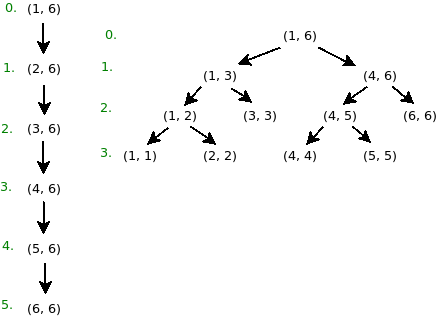
\includegraphics[scale=0.5]{images/prods.png}
\end{center}
\end{figure}

A csomópontokban az egyszerűség kedvéért csak az $(i, j)$ párok vannak feltüntetve. A hívási fák bal oldalán szerepel a verem aktuális szintje.

Az ábrákból leolvasható, hogy az első változatban 5 rekurzív hívás volt, és a maximális veremmélység is 5 volt. A másik esetében 10 rekurzív hívás történt, viszont a maximális veremmélység csak 3.

A rekurzív változat a második esetében lehet előnyös, ha van módunk egymással párhuzamosan számmíttatni a független ágakat. Így a futási idő az elem számának logaritmusával arányosan fog csak növekedni. (A másik esetében ez lineáris növekedést eredményez.)

\end{solution}

\item

Számítsuk ki az $\binom{5}{3}$ értékét!

$$
\binom{n}{k} = \binom{n-1}{k-1} + \binom{n-1}{k}
$$

\item Számítsuk ki a $\sqrt{17}$ értékét az iteratív képletnek megfelelően $\varepsilon = 0.001$ pontosságig!
$$
x_{k+1} = \dfrac{1}{2} \cdot \left( x_k + \dfrac{s}{x_k} \right)
$$

\begin{solution}

\begin{center}
\begin{tabular}{|c|c|c|c|}
$k$ & $x_k$ & $x_k$ kiszámítása & $|x_k - x_{k-1}|$ \\
\hline
0 & 1 & - & - \\
\hline
1 & 9 & $= \dfrac{1}{2} \cdot \left( 1 + \dfrac{17}{1} \right)$ & 8 \\
\hline
2 & 5.444 & $= \dfrac{1}{2} \cdot \left( 9 + \dfrac{17}{9} \right)$ & 3.5556 \\
\hline
3 & 4.2834 & $= \dfrac{1}{2} \cdot \left( 5.444 + \dfrac{17}{5.444} \right)$ & 1.8884 \\
\hline
4 & 4.1261 & $= \dfrac{1}{2} \cdot \left( 4.2834 + \dfrac{17}{4.2834} \right)$ & 0.15729 \\
\hline
5 & 4.1231 & $= \dfrac{1}{2} \cdot \left( 4.1261 + \dfrac{17}{4.1261} \right)$ & 0.003 \\
\hline
6 & 4.1231 & $= \dfrac{1}{2} \cdot \left( 4.1231 + \dfrac{17}{4.1231} \right)$ & 0.000 \\
\hline
\end{tabular}
\end{center}

A 6. lépésben csak az adott pontosságnak megfelelően lesz a két közelítő érték különbsége 0.

\end{solution}

\item

Számítsuk ki a Div\_Sum(1000, $x$) hívás esetén az $x$ értékét!

Div\_Sum(a, @r) \\
// Input: $a \in \mathbb{Z}$ \\
// Output: $r \in \mathbb{Z}$ \\
IF a < 20 \\
\indent \quad THEN $r \leftarrow 0$ \\
\indent \quad ELSE CALL Div\_Sum($a$ DIV 3, $r$) \\
\indent \quad \quad \quad $r \leftarrow r$ + ($a$ DIV 2) + ($a$ DIV 5) \\
RETURN(r)

\begin{solution}

A rekurzív hívási fa a következőképpen néz ki.
\begin{figure}[h!]
\begin{center}
    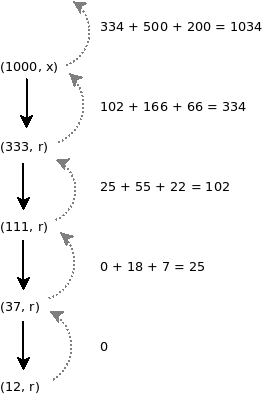
\includegraphics[scale=0.4]{images/divsum.png}
\end{center}
\end{figure}

Az eredmény kiszámításához 4 rekurzív hívásra volt szükség, és a maximális veremmélység is 4 volt.

\end{solution}

\item

Írjunk egy procedúrát, amely egy tömbhöz egy olyan tömböt számol ki, melynek $i$-edik elemén az eredeti tömb $i$-edik utáni elemeinek összege szerepel!

\begin{solution}
\begin{lstlisting}[mathescape]
CUMULATIVE(@X, @Y)
// Input: $X \in \mathbb{R}^n$
// Output: $Y \in \mathbb{R}^n$
Hossz[Y] $\leftarrow$ Hossz[X]
$y_{\text{Hossz[Y]}} \leftarrow 0$
FOR $i \leftarrow$ Hossz[X] - 1 TO 1 DO
	$y_i \leftarrow y_{i + 1} + x_{i + 1}$
RETURN(Y)
\end{lstlisting}
\end{solution}

\end{enumerate}

%=====================
\section*{8. gyakorlat}
%---------------------

\begin{enumerate}

\item Írjunk fel egy rekurzív függvényt a faktoriális kiszámítására!
\begin{itemize}
	\item Számítsuk ki az $5!$ értékét!
	\item Mennyi rekurzív hívás volt a számítás során?
	\item Mekkora volt a maximális mélysége a hívási veremnek?
	\item Rajzoljuk fel a rekurzív hívási fát!
\end{itemize}

\begin{solution}
A rekurzív formula:
$$
n! = \begin{cases}
n \cdot (n - 1)!, & n > 1, \\
1, & n = 1. \\
\end{cases}
$$
Az $5!$ számítása:
$$
5! = 5 \cdot (5 - 1)! = 5 \cdot 4! = 5 \cdot (4 \cdot (4 - 1)!) = 5 \cdot 4 \cdot 3! = 5 \cdot 4 \cdot 3 \cdot 2! = 5 \cdot 4 \cdot 3 \cdot 2 \cdot 1 = 120
$$
A rekurzív függvény pszeudokódja:
\begin{lstlisting}[mathescape]
FACTORIAL(n)
// Input: $n \in \mathbb{N}$
// Output: FACTORIAL
IF $n > 1$
    THEN RETURN($n$ $\cdot$ FACTORIAL($n - 1$)
    ELSE RETURN(1)
\end{lstlisting}

A rekurzív hívási fa \aref{fig:factorial}. ábrán látható.
\begin{figure}[h!]
\begin{center}
    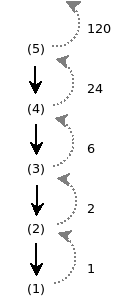
\includegraphics[scale=0.5]{images/factorial.png}
    \caption{Az 5! számítása}
    \label{fig:factorial}
\end{center}
\end{figure}
Ebből leolvasható, hogy 4 rekurzív hívás történt, és a maximális veremmélység is 4 volt.

\end{solution}

\item Számítsuk ki a $\binom{6}{4}$ értékét a rekurzív formula segítségével! Rajzoljuk fel a rekurzív hívási fát!

\item A bináris keresés algoritmusával keressük meg a $10$ értéket a következő tömbben!

$$
A = [1, 4, 5, 10, 11, 13, 14, 16, 17]
$$

\begin{solution}

Az $A$ tömbnek 9 darab eleme van. A bináris keresés algoritmusát célszerű nyílt intervallummal megfogalmazni. Minden lépésben meg kell határozni a középső ($m$) elemet, majd megnézni, hogy az a keresett elemnél kisebb, vagy nagyobb-e, majd annak megfelelően a bal, vagy a jobb oldali részintervallumra folytatni a keresést.

Az $A$ tömb esetében a következő lépésekben történik a keresés. Az $i$ az intervallum elejét, a $j$ az intervallum végét, a $k$ pedig a középső elem indexét jelöli.

\begin{center}
\begin{tabular}{|c|c|c|c|l|}
$i$ & $j$ & $k$ & $m$ & folytatás \\
\hline
0 & 10 & 5 & 11 & bal oldalon \\
0 & 5 & 2 & 4 & jobb oldalon \\
2 & 5 & 3 & 5 & jobb oldalon \\
3 & 5 & 4 & 10 & - \\
\hline
\end{tabular}
\end{center}

\end{solution}

\end{enumerate}

%=====================
\section*{9. gyakorlat}
%---------------------

\begin{enumerate}

\item

Készítsünk egy procedúrát, amely megállapítja, hogy az egy vektor elemei egy adott intervallumba esnek-e!

\begin{solution}
\begin{lstlisting}[mathescape]
BELUL_E(@S, a, b, @belul)
// Input: $S \in \mathbb{R}^n$, valos ertekek vektora
//        $a, b \in \mathbb{R}$ az $[a, b]$ intervallum megadasahoz
// Output: belul $\in$ {igaz, hamis}
$i \leftarrow 1$
WHILE $i \leq$ Hossz[S] and $s_i \geq a$ and $s_i \leq b$ DO
    INC(i)
IF $i$ > Hossz[S]
    THEN belul $\leftarrow$ igaz
    ELSE belul $\leftarrow$ hamis
RETURN(belul)
\end{lstlisting}
\end{solution}

\medskip

Oldjuk meg minimum és maximum számításával is!

\begin{solution}
Tegyük fel, hogy van minimum és maximum érték számításához függvényünk. Ekkor a feladat a következő procedúrával is megoldható.

\begin{lstlisting}[mathescape]
BELUL_E(@S, a, b, @belul)
// Input: $S \in \mathbb{R}^n$, valos ertekek vektora
//        $a, b \in \mathbb{R}$ az $[a, b]$ intervallum megadasahoz
// Output: belul $\in$ {igaz, hamis}
IF MIN(S) $\geq a$ and MAX(S) $\leq b$
    THEN belul $\leftarrow$ igaz
    ELSE belul $\leftarrow$ hamis
RETURN(belul)
\end{lstlisting}

Futási időt tekintve az első változat jobb, mivel csak a szükséges mennyiségű elemet vizsgálja meg. A második megoldás előnye, hogy rövidebb, és így áttekinthetőbb a kód.

\end{solution}

\item

Ellenőrízzük, hogy egy tömb elemei növekvő sorrendben vannak-e!

\begin{solution}
Egy $A$ tömb elemei akkor vannak növekvő sorrendben, ha minden $i$-re teljesül, hogy $a_i \leq a_{i+1}$. Ezt a feltételt ellenőrízni a következőképpen tudjuk.
\begin{lstlisting}[mathescape]
NOVEKVO_E(@A, @novekvo)
// Input: $A \in \mathbb{R}^n$, valos ertekek vektora
// Output: novekvo $\in$ {igaz, hamis}
novekvo $\leftarrow$ igaz
FOR $i \leftarrow 1$ TO Hossz[A] - 1 DO
	IF $a_i > a_{i+1}$
	    THEN novekvo $\leftarrow$ hamis
RETURN(novekvo)
\end{lstlisting}
Ebben az esetben is elképzelhető egy egyszerűbb megoldás, aminél nem szükséges feltétlenül az összes elemet végignézni.
\end{solution}

Vizsgáljuk meg a monoton, és szigorúan monoton eseteket is!

\begin{solution}
A szigorúan monoton esethez csak annyi változtatásra van szükség, hogy a feltételben a $>$ reláció helyett $\geq$ szerepeljen.
\end{solution}

\item

Készítsünk \textit{egy} procedúrát, amely kiszámítja két vektor összegét és skaláris szorzatát!

\begin{solution}
A procedúra például a következő képpen nézhet ki:
\begin{lstlisting}[mathescape]
SUM_SKALAR(@X, @Y, @S, @prod)
// Input: $X, Y \in \mathbb{R}^n$, valos ertekek vektora
// Output: $S \in \mathbb{R}^n$, prod $\in \mathbb{R}$
Hossz[S] $\leftarrow$ Hossz[X]
prod $\leftarrow$ 0
FOR $i \leftarrow 1$ TO $n$ DO
	$s_i \leftarrow x_i + y_i$
	prod $\leftarrow$ prod + $x_i \cdot y_i$
RETURN(S, prod)
\end{lstlisting}
\end{solution}

\item

Írassuk ki egy vektor értékeinek átlagtól való eltérését!

\begin{solution}
Egy lehetséges megoldás:
\begin{lstlisting}[mathescape]
ATLAG_ELTERES(@X, @D)
// Input: $X \in \mathbb{R}^n$, valos ertekek vektora
// Output: $D \in \mathbb{R}^n$ atlagtol elteres
$s \leftarrow 0$
FOR $i \leftarrow 1$ TO $n$ DO
    $s \leftarrow s + x_i$
atlag $\leftarrow s / n$
Hossz[D] $\leftarrow$ Hossz[X]
FOR $i \leftarrow 1$ TO $n$ DO
    $d_i \leftarrow x_i - \text{atlag}$	
RETURN(D)
\end{lstlisting}
\end{solution}

\item

Ellenőrízzük, hogy egy vektor minden eleme különböző!

\begin{solution}
Függvény az ellenőrzéshez:
\begin{lstlisting}[mathescape]
MIND_KULONBOZO(@X)
// Input: $X \in \mathbb{R}^n$, valos ertekek vektora
// Output: MIND_KULONBOZO $\in$ {igaz, hamis}
FOR $i \leftarrow 1$ TO $n$ DO
    FOR $j \leftarrow 1$ TO $n$ DO
        IF $i \neq j$
            THEN IF $x_i = x_j$
                    THEN MIND_KULONBOZO $\leftarrow$ hamis
                         RETURN
MIND_KULONBOZO $\leftarrow$ igaz
RETURN
\end{lstlisting}
\end{solution}

\item

Hogyan tudnánk bekérni, tárolni és kiíratni egy alsóháromszögmátrix értékeit?

\begin{solution}
A bekérést, tárolást és kiíratást oldjuk meg egy procedúrával, amelynek a bemenete a mátrix sorainak száma lesz. Az elemeket egy $A$ tömbben tároljuk.
\begin{lstlisting}[mathescape]
HAROMSZOG_MATRIX(n)
// Input: $n$, a matrix sorainak a szama
// Adatbekeres es tarolas
Hossz[A] $\leftarrow (n \cdot (n + 1)) / 2$
$k \leftarrow 0$
FOR $i \leftarrow 1$ TO $n$ DO
    FOR $j \leftarrow 1$ TO $i$ DO
        INC($k$)
        INPUT($a_k$)
// Matrix elemeinek kiiratasa
$k \leftarrow 0$
FOR $i \leftarrow 1$ TO $n$ DO
    FOR $j \leftarrow 1$ TO $n$ DO
        IF $i \leq j$
            THEN INC($k$)
                 OUTPUT($a_k$)
            ELSE OUTPUT(0)
    OUTPUT('\n')
\end{lstlisting}
\end{solution}

\item

Vizsgáljuk meg, hogy egy mátrix szimmetrikus-e!

\begin{solution}
\begin{lstlisting}[mathescape]
SZIMMETRIKUS_E(@A)
// Input: $A \in \mathbb{R}^{n \times n}$
// Output: SZIMMETRIKU_E $\in$ {igaz, hamis}
FOR $i \leftarrow 2$ TO $n$ DO
    FOR $j \leftarrow 1$ TO $i - 1$ DO
        IF $a_{ij} \neq a_{ji}$
            THEN SZIMMETRIKUS_E $\leftarrow$ hamis
                 RETURN
SZIMMETRIKUS_E $\leftarrow$ igaz
RETURN
\end{lstlisting}
\end{solution}

\item

Fordítsuk meg egy vektor elemeinek a sorrendjét!

\begin{solution}
\begin{lstlisting}[mathescape]
FORDIT(@X)
// Input: $X \in \mathbb{R}^{n}$
// Output: Az $X$ forditott sorrendben
FOR $i \leftarrow 1$ TO $\left \lfloor \dfrac{n}{2} \right \rfloor$ DO
    $k \leftarrow n - i + 1$
    $t \leftarrow x_i$
    $x_i \leftarrow x_k$
    $x_k \leftarrow t$
RETURN(X)
\end{lstlisting}
\end{solution}

\item

Transzponáljuk egy mátrix elemeit!

\medskip

Vizsgáljuk meg a segédmátrixos és helyben transzponálós változatot is!

\begin{solution}

A segédmátrixos változat:
\begin{lstlisting}[mathescape]
TRANSPOSE(@A, @B)
// Input: $A \in \mathbb{R}^{n \times n}$
// Output: $B \in \mathbb{R}^{n \times n}$
FOR $i \leftarrow 1$ TO $n$ DO
    FOR $j \leftarrow 1$ TO $n$ DO
        $b_{ij} \leftarrow a_{ji}$
RETURN(B)
\end{lstlisting}

A helyben transzponálós változat:
\begin{lstlisting}[mathescape]
TRANSPOSE(@A)
// Input: $A \in \mathbb{R}^{n \times n}$
// Output: $A \in \mathbb{R}^{n \times n}$
FOR $i \leftarrow 2$ TO $n$ DO
    FOR $j \leftarrow 1$ TO $i - 1$ DO
        $t \leftarrow a_{ij}$
        $a_{ij} \leftarrow a_{ji}$
        $a_{ji} \leftarrow t$
RETURN(A)
\end{lstlisting}

Egy CSERE függvény használatával az utóbbi változat áttekinthetőbbé tehető.

\end{solution}

\item

Egy egész értékeket tároló vektorban keressünk Pithagoraszi számhármasokat, vagyis amelyekre teljesül, hogy $x^2 + y^2 = z^2$.


\begin{solution}
\begin{lstlisting}[mathescape]
PITHAGORASZ(@S)
// Input: $S \in \mathbb{R}^{n}$
FOR $i \leftarrow 1$ TO $n$ DO
    FOR $j \leftarrow 1$ TO $n$ DO
        FOR $k \leftarrow 1$ TO $n$ DO
            IF $s_i^2 + s_j^2 = s_k^2$
                THEN OUTPUT(s_i, s_j, s_k)
RETURN
\end{lstlisting}

\end{solution}

\end{enumerate}

%=====================
\section*{10. gyakorlat}
%---------------------

Síkbeli pontok adatait tároljuk egy tömbben $(x, y)$ rendezett párok formájában folytonosan.

$$ [
\begin{array}{ccccccccc}
x_0 & y_0 & x_1 & y_1 & \ldots & x_{n-1} & y_{n-1} & x_n & y_n
\end{array}
] $$

\noindent \textit{Mennyi eleme lesz a vektornak $n$ pont esetén?}

\begin{enumerate}

\item

Írassuk ki a koordináták mellé, hogy melyik pont melyik síknegyedbe esik!

\item

Toljuk el az összes pontot egy adott vektorral!

\item

Írassuk ki azon pontok koordinátáit, amelyek az origó $r$ sugarú környezetébe esnek!

\item

Keressük meg a két legközelebbi és legtávolabbi pontot!

\item

Határozzuk meg annak a legkisebb téglalapnak a bal felső és jobb alsó pontjának koordinátáit, amelynek oldalai a tengelyekkel párhuzamosak!

\item

Keressük meg azon pontokat, amelyek egy egyenesbe esnek!

\item

Általánosan hogy kereshetnénk legkisebb területű téglalapot, négyzetet, kört?

\item

Készítsünk egy procedúrát, amely egy szöveges értékről megállapítja, hogy az lehet-e email cím!

\item

Vágjunk ki egy sztringből egy adott részt!

\item

Konkatenáljunk össze két sztringet!

\item

Távolítsuk el egy szövegből a szóközöket!

\medskip

Módosítsuk a programot, hogy csak a felesleges/duplikált szóközök kerüljenek eltávolításra!

\end{enumerate}

%======================
\section*{11. gyakorlat}
%----------------------

\begin{enumerate}

\item 

Soroljuk fel a 12 elemi algoritmust!

\item

Mik a jó program ismérvei?

\item

Mik a struktúrált programok alapelemei?

\medskip

Rajzoljuk fel a szekvencia, a ciklus és az elágazás folyamatábráját/programgráfját, illetve írjuk fel a formulájukat és pszeudókódjaikat!

\item

Adjuk meg a teljes, és a tömör élhalmazos felírását a következő gráfoknak!

// TODO: A gráfot még meg kell rajzolni!

teljes
\begin{gather*}
P = \{(START, A), (A, B), (B, C), (C, D/i), (D, E/i), (D, F/h), (E, G), \\
(F, G), (G, H), (H, B), (C, I/h), (I, STOP)\}
\end{gather*}

tömör
\begin{gather*}
P = \{START \rightarrow A, A \rightarrow C, C \rightarrow (D, I), D \rightarrow (E, F), \\
E \rightarrow H, F \rightarrow H, H \rightarrow C, I \rightarrow STOP\}
\end{gather*}

\item

Rajzoljuk fel a programgráfot az élhalmaz alapján!

\begin{gather*}
P = \{
(START, A), (A, B), (B, C/i), (B, G/h), (G, H), (H, I),\\
(C, D), (D, E), (E, F/i), (E, I/h), (I, J), (J, STOP)
\}
\end{gather*}

\item

Rajzoljuk fel a programgráfot a pszeudókód alapján!

\begin{verbatim}
N: A
    IF B
        THEN C
        ELSE GOTO N
\end{verbatim}

\item

Rajzoljuk fel a programgráfot, és adjuk meg az ekvivalens struktúrált programgráfot!

\begin{gather*}
P = \{
START \rightarrow A, A \rightarrow (B, C), B \rightarrow (S1, S2), C \rightarrow (S2, S3), \\
S1 \rightarrow D, S2 \rightarrow D, S3 \rightarrow D, D \rightarrow STOP
\}
\end{gather*}

\item

Mit nevezünk ciklikus bonyolultságnak, és lényeges bonyolultságnak?

$$
m(P) = e - c, \quad
m(P) = p + 1, \quad
M(P) = m(P) - k
$$

\end{enumerate}

%======================
\section*{12. gyakorlat}
%----------------------

\begin{enumerate}

\item

Adjunk példákat nem valódi programok programgráfjára, amelyek csak adott kritériumoknak nem felelnek meg!

\begin{solution}
Kritériumok:
\begin{itemize}
\item Véges számú, nem zérus be- és kimeneti éllel rendelkezik.
\item A programgráf csomópontjai predikátumok, függvények és gyűjtők.
\item A programgráf minden csomópontján keresztül vezet legalább egy útvonal, amely egy bemenő éllel és egy kimenő éllel rendelkezik.
\end{itemize}
\end{solution}

\item

A következő, tömör élhalmazos formában megadott programokhoz készítsünk
\begin{itemize}
	\item programgráfot
	\item írjuk fel a formuláját
	\item Írjuk fel az eredeti és a struktúrált program pszeudó kódját
	\item Számítsuk ki a ciklikus bonyolultságot
	\item Rajzoljuk fel a struktogramot
\end{itemize}

$$
P = \{START \rightarrow A, A \rightarrow (B, C), B \rightarrow (D, E), C \rightarrow E, D \rightarrow A, E \rightarrow STOP\}
$$

$$
P = \{START \rightarrow A, A \rightarrow B, B \rightarrow (C, D), C \rightarrow B, D \rightarrow E, E \rightarrow (A, STOP)\}
$$

$$
P = \{START \rightarrow A, A \rightarrow B, B \rightarrow (C, D), C \rightarrow B, D \rightarrow C, E \rightarrow (A, STOP)\}
$$

$$
P = \{START \rightarrow A, A \rightarrow (B, C), B \rightarrow D, C \rightarrow E, D \rightarrow (A, F), E \rightarrow (A, F), F \rightarrow STOP\}
$$

$$
P = \{
START \rightarrow A, A \rightarrow (B, C), B \rightarrow (D, E), C \rightarrow A, D \rightarrow A, E \rightarrow (D, STOP)
\}
$$

$$
P = \{
START \rightarrow A, A \rightarrow (B, C), B \rightarrow (D, E), C \rightarrow E, D \rightarrow A, E \rightarrow STOP
\}
$$

$$
P = \{
START \rightarrow A, A \rightarrow B, B \rightarrow (C, D), C \rightarrow (B, STOP), D \rightarrow (C, A)
\}
$$

$$
P = \{
START \rightarrow A, A \rightarrow (B, E), B \rightarrow C, C \rightarrow (D, G), D \rightarrow A, E \rightarrow (F, STOP), F \rightarrow G, G \rightarrow STOP
\}
$$

$$
P = \{
START \rightarrow A, A \rightarrow (D, B), B \rightarrow C, C \rightarrow (E, STOP), D \rightarrow F, E \rightarrow A, F \rightarrow (B, C)
\}
$$

\item

A pszeudókódok alapján rajzoljuk fel a programgráfot, majd készítsük el az ekvivalens struktúrált programokat.

\begin{verbatim}
1 IF A
2   THEN B
3       IF C
4           THEN F
5           ELSE GOTO 8
6   ELSE
7       WHILE D DO
8           E
9 G
\end{verbatim}

\begin{verbatim}
1 IF A
2   THEN
3       WHILE B DO
4           C
5       GOTO 10
6   ELSE
7       IF D
8           THEN
9               DO E
10                  WHILE F
11          ELSE G
\end{verbatim}

\begin{verbatim}
1 IF A
2   THEN
3       B
4       IF D
5           THEN GOTO 7
6   ELSE
7       C
8       IF E
9           THEN GOTO 3
\end{verbatim}

\item

Keressük meg egy valós értékeket tartalmazó tömbben egy procedúrával a paraméterként kapott $z$ értékhez a legközelebbi elemet!

\item

Válogassuk szét egy valós tömb elemeit negatív és nemnegatív értékekre!

\item

Töröltjük egy tömbből a 0 értékű elemeket! \textit{(a. segédtömbbel, b. segédtömb nélkül)}

\item

Írjunk egy procedúrát, amely 2, azonos méretű valós értékeket tároló tömbhöz visszaadja az adott indexeken lévő minimális értékeket.

pl.: $x = [5, 8, -1], y = [2, 1, 3] \Rightarrow z = [2, 1, -2]$

\item

Számítsuk ki két vektor különbségének négyzetösszegét!

\end{enumerate}

%======================
\section*{13. gyakorlat}
%----------------------

\textit{COCOMO modell}

\begin{itemize}
    \item PM: Person Month
    \item $T_d$: Development Time
    \item KDSI: Kilo Delivered Source Index
\end{itemize}

$$
PM = 2.4 \cdot KDSI^{1.05},
\quad
T_d = 2.5 \cdot \sqrt[3]{PM},
\quad
\text{létszám} = \dfrac{PM}{T_d},
\quad
\text{Brook limit}: T_d \cdot 0.75
$$

\begin{enumerate}

\item Egy 100000 soros alkalmazást szeretnénk kifejleszteni. Mennyi emberre és időre van szükség?

\item 20 programozóval fél év alatt mekkora alkalmazást lehet kifejleszteni?

\item Egy 300000 soros program esetében lehetőségünk van egy függvénykönyvtár megvásárlására, amely 120000 sor kiváltására képes.

\medskip

Maximum mennyit érdemes fizetnünk ezért, ha a programozók havi fizetése 240000 Ft?

\item Egy 50000 soros alkalmazást szeretnénk minél gyorsabban elkészíteni. Mennyi plusz embert lehet még bevonni, hogy a határidő tartása ne legyen rizikós?

\item Egy 1000000 soros alkalmazást 25 emberrel szeretnénk kifejleszteni. Az alkalmazást várhatóan 5 millió forintént fog elkelni.

\medskip

Legfeljebb mennyi lehet így a programozók havi fizetése?

\item

Írjuk át iteratív alakra a következő rekurzív algoritmust!

Parity(x, @y) \\
// Input: $x \in \mathbb{N}$ \\
// Output: $y \in \mathbb{N}$ \\
IF x = 0 \\
\indent \quad THEN y $\leftarrow$ 1 \\
\indent \quad ELSE IF x mod 2 = 0 \\
\indent \quad \quad THEN CALL Parity(x-1, y) \\
\indent \quad \quad \quad \quad \quad y $\leftarrow$ y + x \\
\indent \quad \quad ELSE CALL Parity(x-1, y) \\
\indent \quad \quad \quad \quad \quad y $\leftarrow$ y $\cdot$ x \\
RETURN(y)

\item

Írjuk át iteratív alakra a következő rekurzív algoritmust!

ADDER(@X, i, @a, @b) \\
// Input: $X \in \mathbb{R}, i \in \mathbb{N}$ \\
// Output: $a, b \in \mathbb{R}$ \\
IF i > 0 \\
\indent \quad THEN \\
\indent \quad \quad ADDER(X, i - 1, a, b) \\
\indent \quad \quad IF $x_i$ > 0 \\
\indent \quad \quad \quad THEN a $\leftarrow$ a + $x_i$ \\
\indent \quad \quad \quad ELSE b $\leftarrow$ b + $x_i$ \\
\indent \quad ELSE \\
\indent \quad \quad a $\leftarrow$ 0 \\
\indent \quad \quad b $\leftarrow$ 0 \\
RETURN(a, b)

\item

Írjuk át iteratív alakra a következő rekurzív algoritmust!

TRNG(x, @y) \\
// Input: $x \in \mathbb{R}$ \\
// Output: $y \in \mathbb{R}$ \\
IF x > 0 \\
\indent \quad THEN FOR i $\leftarrow$ 1 TO X DO \\
\indent \quad \quad \quad \quad \quad CALL TRNG(x-1, y) \\
\indent \quad \quad \quad \quad \quad INC(y) \\
\indent \quad ELSE y $\leftarrow$ 0 \\
RETURN(y)

\item

Készítsünk egy algoritmust, amely úgy osztályozza a tömbben tárolt egészeket, hogy a párosakat a tömb elejére, a páratlanokat a tömb végére helyezi.

\item

Készítsünk algoritmust, amely $k$ szerinti maradékosztályok szerint rendezi egy tömb elemeit, vagyis az egyes szakaszok értékeit $k$-val osztva $0, 1, \ldots k-1$ maradékot adnak.

\medskip

Például 4 esetén:

$$
[1, 5, 9, 7, 4, 3, 1, 2, 8, 6, 5] \quad \rightarrow \quad [4, 8, 1, 5, 9, 1, 5, 2, 6, 7, 3]
$$

\item

Írassuk ki egy vektor elemeinek összes lehetséges permutációját!
\begin{itemize}
    \item[a.] Rekurzív algoritmussal
    \item[b.] Iteratív algoritmussal
\end{itemize}

\item

Számítsuk ki, hogy egy vektorban melyik értékből mennyi van.
\begin{itemize}
    \item[a.] Természetes számokat tároló vektor előre rögzített maximális értékkel
    \item[b.] Tetszőleges elemtípusra vektorok vektorával
\end{itemize}

\end{enumerate}

%======================
\section*{14. gyakorlat}
%----------------------

\textit{Az eddigi feladatok gyakorlása.}


\section*{Kimaradt feladatok}

\begin{enumerate}

\item

Mik lesznek a következő halmazok elemei?

\begin{itemize}
    \item $\{x \in \mathbb{R} : x^2 - 2 = 0\}$
    \item $\{x \in \mathbb{R} : 2\log x = \log x^2\}$
    \item $\{x \in \mathbb{R} : 1 < |x| \leq 5\}$
    \item $\{(x, y) \in \mathbb{R}^2 : x^2 + y^2 = 4 \text{ és } y \geq 0\}$
    \item $\{(x, y) \in \mathbb{R}^2 : |x| < y \leq 1\}$
\end{itemize}

\item

Milyen halmazok esetén állnak fenn a következő egyenlőségek?

\begin{itemize}
    \item $(A \setminus X) \cap (B \setminus X) = A$
    \item $(A \cap B) \cup X = X$
    \item $(A \cap X) \cup B = X$
    \item $A \setminus X = X \setminus A$
\end{itemize}

\item

Milyen elemek tartoznak a következő halmazokhoz?

\begin{itemize}
    \item $\{(a, b) \in \mathbb{N}^2 | a \mod b = 6, a + b = 20\}$
    \item $\{(a, b) \in \mathbb{N}^2 | a \text{ div } b = 3, a \cdot b < 50\}$
    \item $\{(x, y) \in \mathbb{R}^2 : \text{Round}(x) + \text{Round}(y) = 3\}$
    \item $\{(x, y) \in \mathbb{R}^2 : \{x\} > \{y\}\}$
\end{itemize}

\item

Igazoljuk, hogy $(p \wedge q) \rightarrow q \equiv p \rightarrow (p \vee \overline{q})$ kifejezéssel!

\item

Mivel egyenlő az $A \bigtriangleup B \bigtriangleup C$ kifejezés?

\begin{solution}
Előtte be kell látni, hogy kommutatív a kifejezés!
\end{solution}

\item

Egy sportegyesületnek 550 tagja van. A tagok 20\% -a kajakozik, vagy kenuzik. A tagok közül 60-an kajakoznak és 25-en mind a két sportot űzik. Hányan kenuznak?

\item

Egy matematika versenyen 2 feladatot tűztek ki. Az elsőt az indulók 80\%-a, a másodikat a 40\%-a oldotta meg. Minden résztvevő megoldott legalább 1 feladatot, mindkét feladatot ketten oldották meg. Hányan indulhattak a versenyen?

\item

Egy faluban 1000 ház van. Ezek közül 250-ben van autó, 900-ban hűtőszekrény, 950-ben televízió és 990-ben rádió. Legalább mennyi házban van mind a négy?

\item

Készítsünk egy olyan függvényt, amely a 3 paraméter értékéből a középső elem értékével tér vissza! (med(a, b, c) ...)

\end{enumerate}

\end{document}
